The server is the central part of the whole system. It is here the Raspberry PIs send all the gathered data, where data are stored and structured, and where Android devices can fetch information about rooms, people, and predictions on which exits a person is most likely to use.

All sorts of devices can be used to capture and process data. To simplify the process and to allow access for all types of devices, the server provides an API which allows the senders to focus on data capturing and processing.

As with the devices providing the data for the server, the devices which requests data from the server can be of different types. By providing an API these devices can focus on how to use and present the data, and let the server focus on how the data is fetched. This ensures that all data is available for everyone and that each request has a minimum of effect on other devices access to the data.

When data is received the server will store it in a database, making it easier to get relevant data for both positioning of occupants and predictions. An outline of the database is seen in figure~\ref{fig:database_er_diagram} 

\begin{figure}[htb]
	\centering
	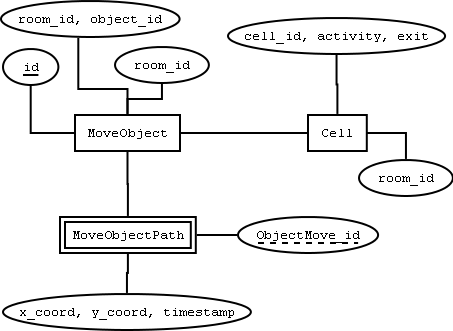
\includegraphics[scale=0.70]{server/ER}
	\caption{Database ER Diagram}
	\label{fig:database_er_diagram}
\end{figure}

The entity "ObjectMove" keeps track of all objects, storing which camera has captured the position and in which room. The entity "ObjectMovePath" keeps track of where each object has been located and at which time, and the entity "Cells" keeps track of how often a given position has been visited and which positions are considered exits.